%% The following is a directive for TeXShop to indicate the main file
%%!TEX root = diss.tex

\chapter{Introduction}
\label{ch:Introduction}

\section{Incidence and mortality of breast cancer}
Breast cancer is the most common type of cancer in Canadian women behind non-melanoma skin cancers and is the second highest cause of cancer related deaths in women. In 2020, 27,400 women will be diagnosed and 5,100 women will die from breast cancer. On average, 75 Canadian women will be diagnosed while 14 Canadian women will die from breast cancer every day. Among females, the age-standarized incidence rates (ASIR) for breast cancer rose between 1984 and the early 1990s after which it has fluctuated and the age-standarized mortality rates (ASMR) has decreased consistently for breast cancer \cite{canadian2020canadian} \textbf{\autoref{fig:breastcancerstats}}.

\begin{figure}
\centering
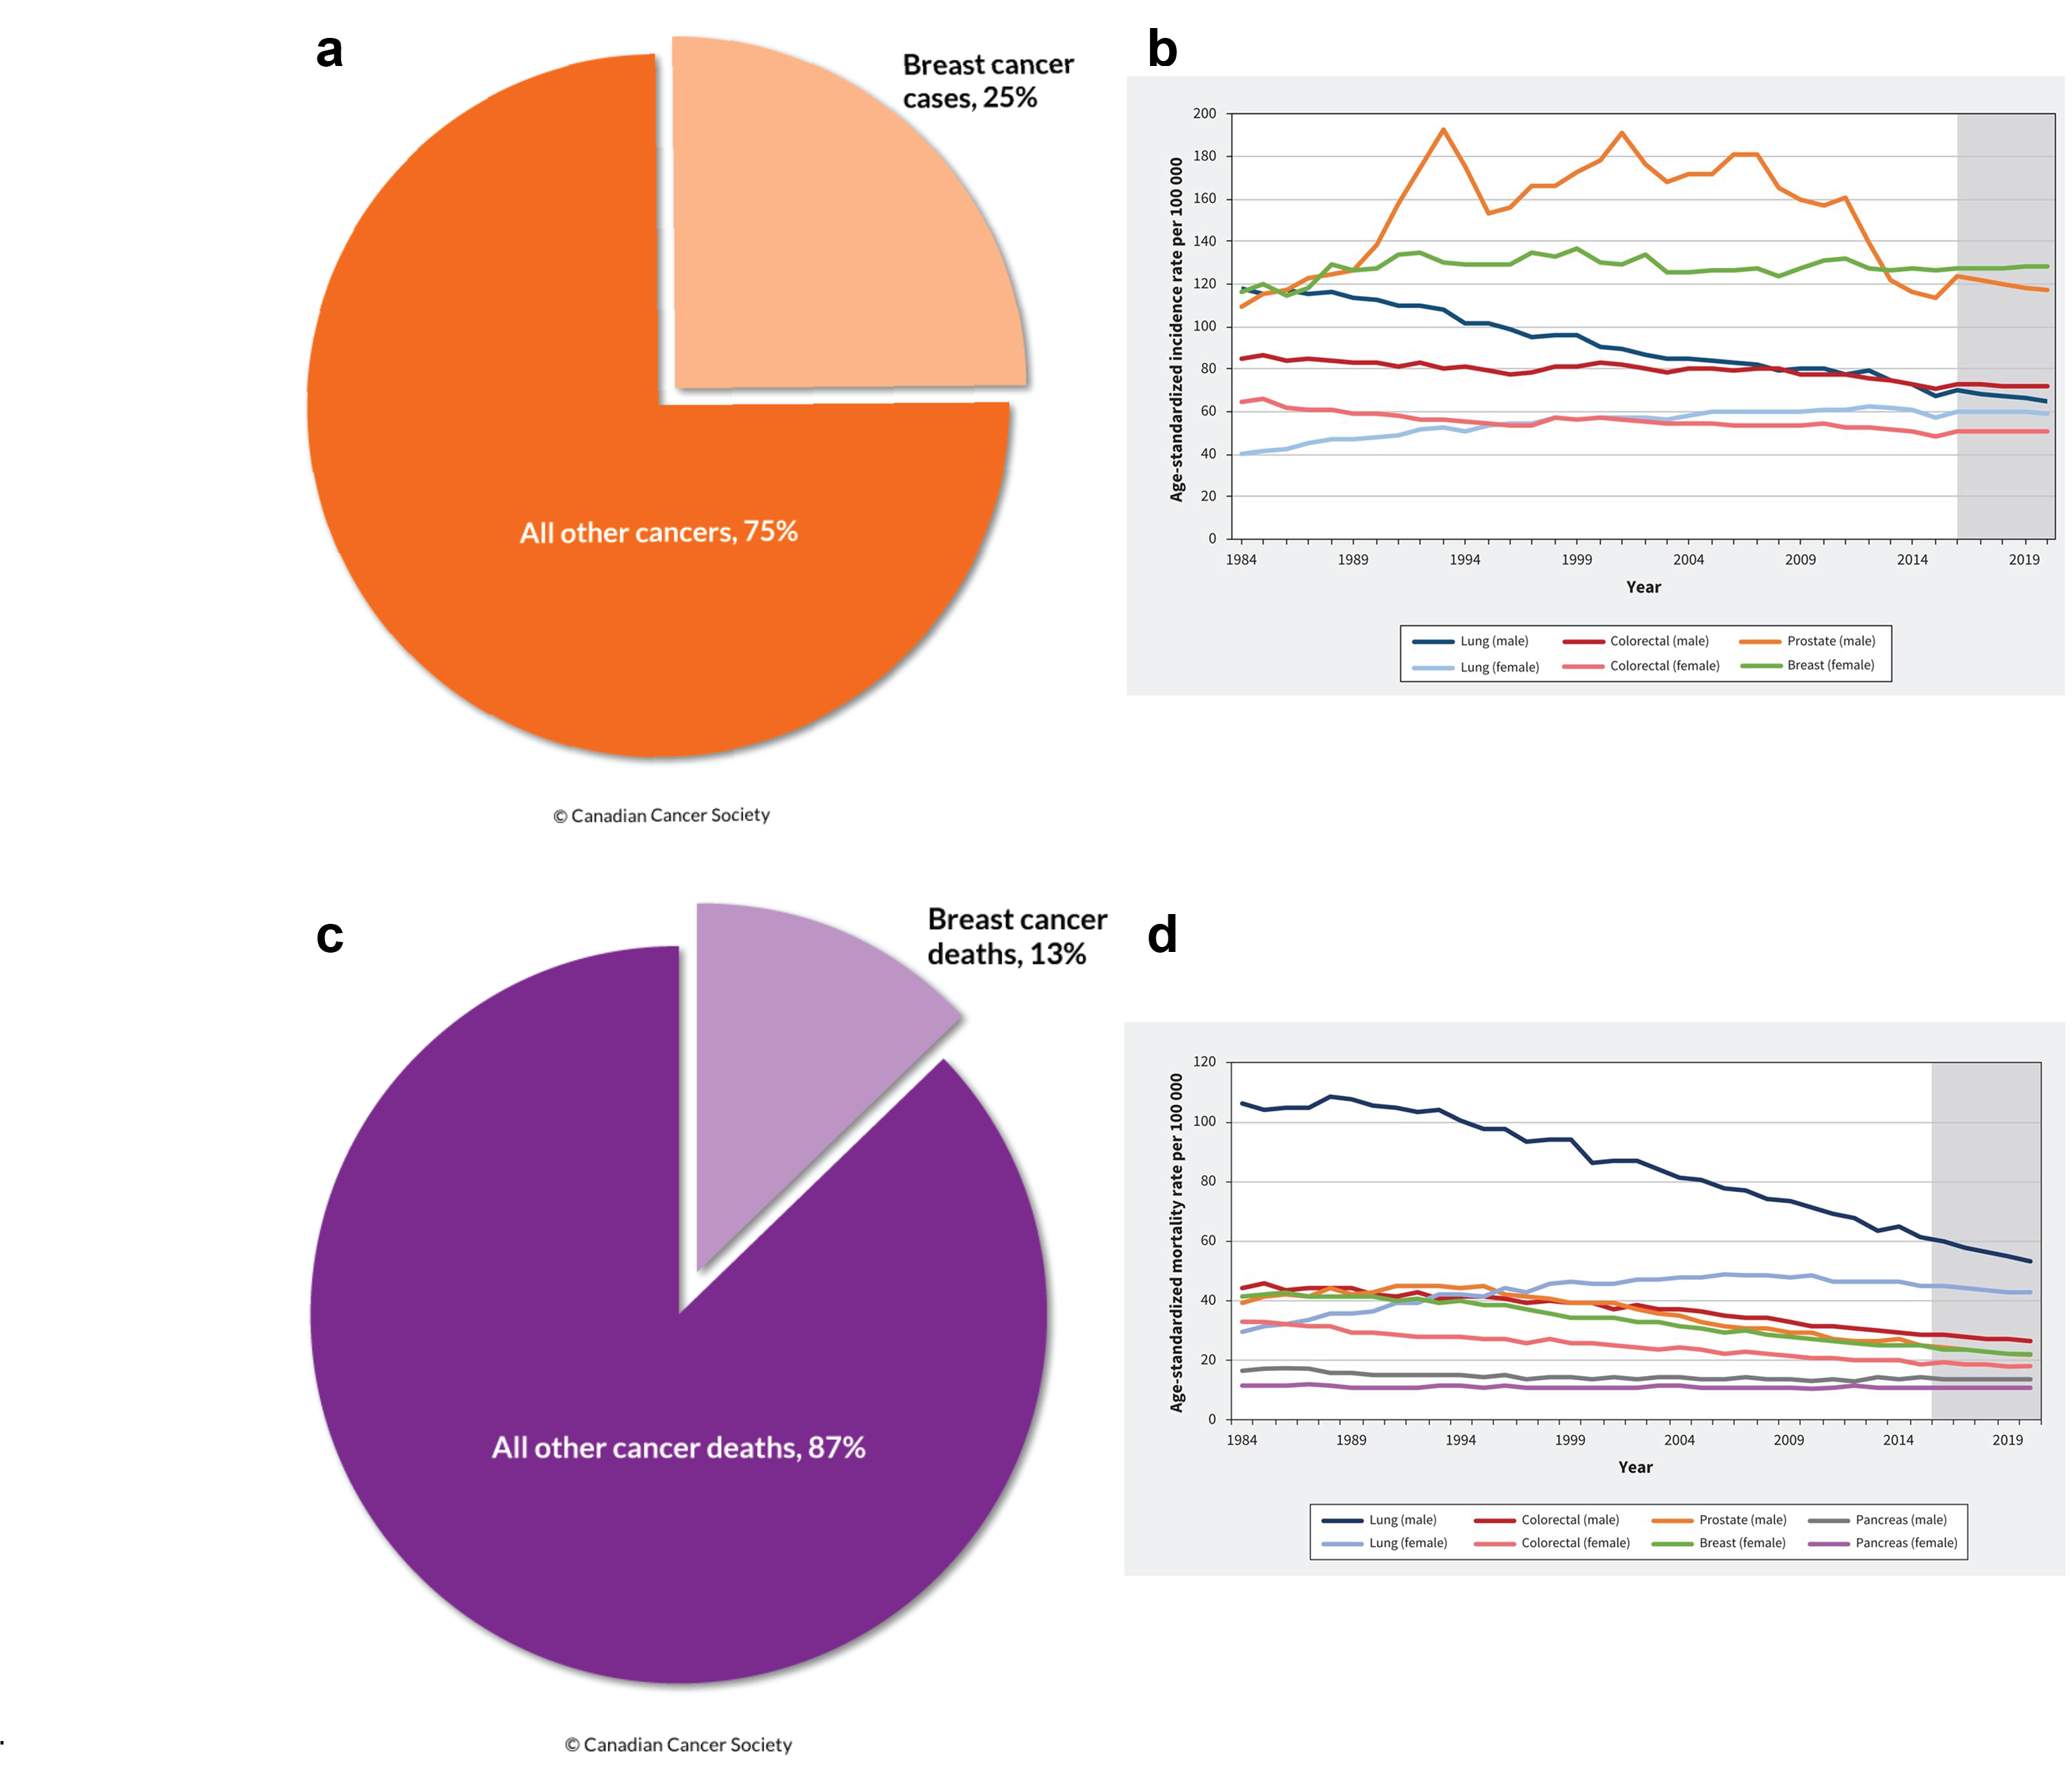
\includegraphics[width=\textwidth]{Figures/breastcancerstats.png}
	\caption[Breast cancer statistics by Canadian cancer society ]
	{\small
	    \textbf{Breast cancer statistics by Canadian Cancer Society.}
	    \textbf{(a)}, Percentage of all estimated new cancer cases in women in 2020.
	    \textbf{(b)}, Age-standardized incidence rates (ASIRs) for selected cancers, in Canada (excluding Quebec), 1984–2020, by sex. Shading indicates projected data.
	    \textbf{(c)}, Percentage of all estimated cancer deaths in women in 2020
	     \textbf{(d)},Age-standardized mortality rates (ASMRs) for selected cancers in Canada, 1984–2020, by sex. Shading indicates projected data.
	}
	\label{fig:breastcancerstats}
\end{figure}

%%%%%%%%%%%%%%%%%%%%%%%%%%%%%%%%%%%%%%%%%%%%%%%%%%%%%%%%%%%%%%%%%%%%%%

\section{Breast cancer heterogeneity}
It is well acknowledged that there are both genetic and functional differences between tumours. Tumours that originate from different tissues and cells diversify in terms of their genomic as well as transcriptomic landscapes, prognosis and their response to cytotoxic therapies, probably resulting from the fact that the genetic events of transformation interact with cell-intrinsic biological properties.Following this, site of origin plays an important role in treatment decision.However, genomic aberrations, aggressiveness, phenotypic characteristics and drug sensitivity is also observed between tumours that originate from the same tissue and cell type \cite{vogelstein2013cancer}. This tumor state of being diverse is known as heterogeneity.
Tumor heterogeneity makes every cancer a unique disease. Heterogeneity occurs at various levels in malignant carcinomas. Inter tumor heterogeneity or population heterogeneity refers to the exclusiveness of the same type of cancer in different patients. That is, each patient's tumor is unique, despite of sharing some properties. The presence of distinct subpopulations of cells within a tumor with distinguishable genotypic and phenotypic differences was classically demonstrated several decades ago \cite{fidler1978tumor}.
The concept of intratumor heterogeneity implies to the presence of heterogeneous cell populations within an individual tumor that includes both spatial and temporal factors following variability over time during tumor growth \cite{ellsworth2017molecular, welch2016tumor}. Inter and intratumour heterogeneity have significant implications for the choice of chemotherapy to govern clinical decision-making in cancer medicine \cite{bedard2013tumour}.


\begin{figure}
\centering
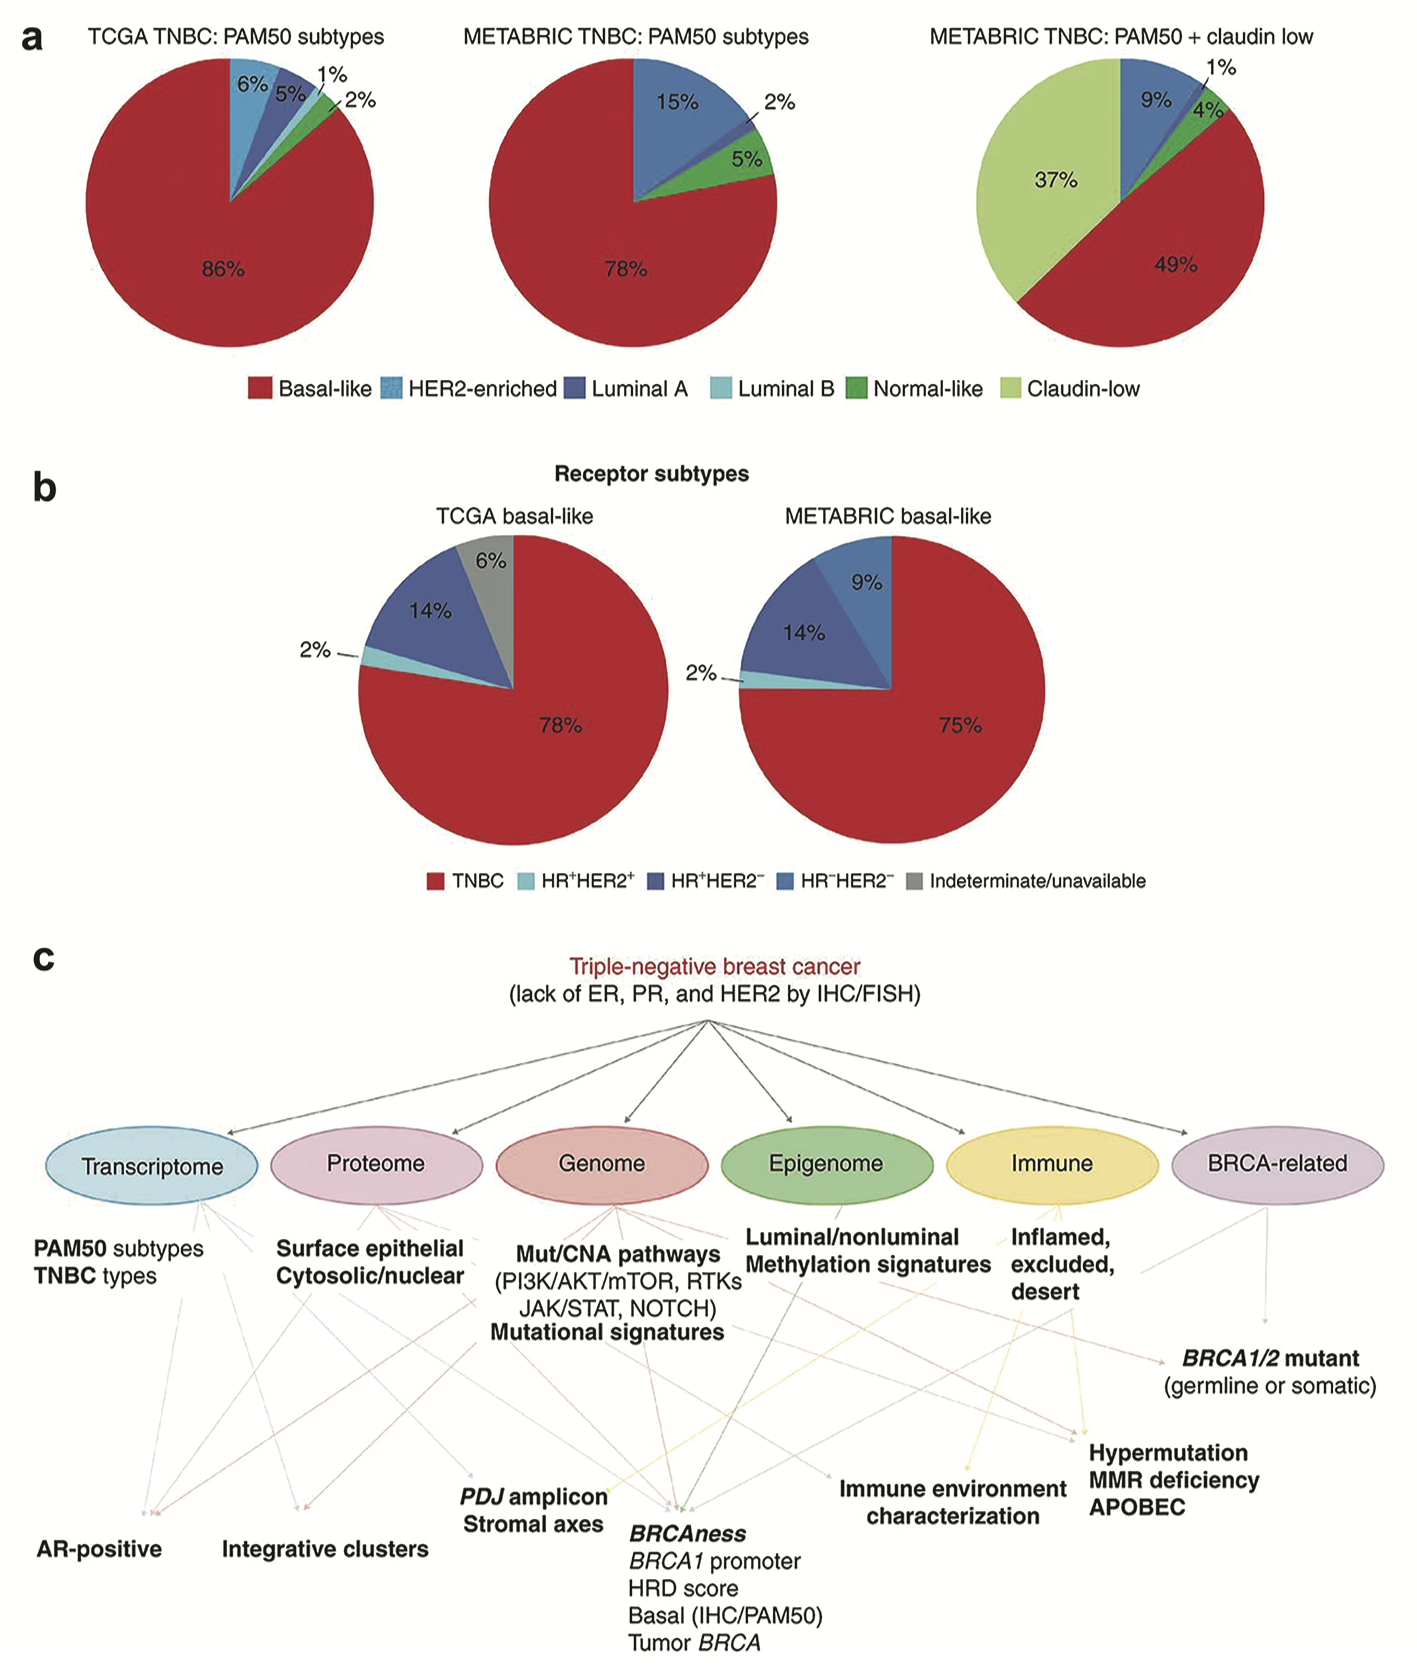
\includegraphics[width=\textwidth]{Figures/Breastcancersubtypes.png}
	\caption[Breast cancer subtypes]
	{\small
	    \textbf{Breast cancer subtypes adapted from \cite{garrido2019insights}.}
	    \textbf{(a)}Intrinsic subtypes defined by PAM50 and PAM50 + claudin-low in The Cancer Genome Atlas (TCGA) and METABRIC data sets in \ac{TNBC}.
	    \textbf{(b)} Distribution of breast cancer subtype according to receptor status defined by IHC in TCGA and METABRIC data sets in basal-like breast cancer.
	    \textbf{(c)} Interactions among molecular classifications of TNBC based on genomic, transcriptomic, proteomic, epigenomic, and immune characterization of the tumor and its microenvironment. ER, estrogen receptor; PR, progesterone receptor; Mut, mutant; RTK, receptor tyrosine kinase; MMR, mismatch repair; CNA, copy-number alteration; AR, androgen receptor; HRD, homologous recombination deficiency; IHC, immunohistochemistry.
	}
	\label{fig:Breastcancersubtypes}
\end{figure}




\subsection{Hormone receptor status in breast cancer}

The estrogen receptor (ER), progesterone receptor (PR), and ERBB2 also known as human epidermal growth factor receptor 2 (HER2) is routinely determined in all invasive breast carcinomas by immunohistochemistry (IHC) as recommended by cancer control committees and unions \cite{turashvili2017tumor, hammond2010college, wolff2013american}. These are categorized as subtypes of breast cancer and are characterized by their molecular profiles, morphology, and expression of specific biomarkers. The receptor status in the growing tumors also creates another complex layer of intra tumor heterogeniety. For example, some cells that express the ER in breast tumors varies from 1 to 100\% cells in the tumor.\cite{januvskevivciene2019heterogeneity, visvader2011cells}. These receptors are actionable targets for treatments such as hormone therapies with drugs like tamoxifen, a non-steroidal antiestrogen used to treat estrogen receptor positive breast cancers \cite{jordan2003tamoxifen,fisher2005tamoxifen} and monoclonal antibodies such as herceptin that targets overexpressed ERBB2 (HER2), which have proven to be effective \cite{piccart2005trastuzumab,slamon2011adjuvant}.  
For the scope of this thesis We have worked with three triple negative breast cancers (Chapter 4, 5) and one HER2+ (Chapter 4) breast cancer.



\begin{figure}
\centering
\includegraphics[width=\textwidth]{Figures/TNBChistologicsubtypes.png}
	\caption[TNBC histologic subtypes adapted from a rev \cite{bianchini2016triple} ]
	{\small
	    \textbf{TNBC histologic subtypes adapted from a review  \cite{bianchini2016triple}.}
	    \textbf{(a)}, Histological subtypes. Some rare but relevant subtypes are shown for
illustrative purposes.
	    \textbf{(b)}, Gene-expression-based subtypes of triple-negative breast cancer (TNBC) according to PAM50 \cite{prat2013molecular}.
	    \textbf{(c)}, Gene-expression-based subtypes defined by Lehmann \textit{et al}.\cite{lehmann2011identification}
	     \textbf{(d)} Integrative clusters (IntClust) of genomic and transcriptomic data applied to basal-like breast cancer (BLBC) defined by gene-expression.
	     \textbf{(e)} Heterogeneity of tumour infiltrating lymphocytes. Tumours with low, intermediate and high lymphocyte infiltration are shown for illustrative
purposes. BL1, basal-like 1; BL2, basal-like 2; IM, immunomodulatory; LAR, luminal androgen receptor; M, mesenchymal;
MSL, mesenchymal stem-like; UNC, unclassified; UNS, unstable.
	}
	\label{fig:TNBChistologicsubtypes}
\end{figure}



\subsection{Insights into triple negative breast cancer heterogeneity}
Patient grouping defined by the absence of biomarkers ER, PR, and HER2, usually referred to as “triple-negative” breast cancers (TNBC). It constitutes an extremely heterogeneous group with regard to histology, genetic diversity and treatment resulting in poor prognosis. TNBC accounts for $\approx$~15\% to 20\% of newly diagnosed breast cancers \cite{reis2008triple}.
The overall survival rate of TNBC is shorter as compared to other breast cancer subtype and the mortality rate within first 5 years is 40\%. The recurrance rate in TNBC after surgery is  around 25\% with distant metastasis developing in three years of diagnosis. Unfortunately, the median survival rate after metastasis is only 13.5 months \cite{dent2007triple,lin2008sites} so there is a critical need to understand the extent and mechanisms of heterogeneity in TNBC that results in treatment outcome. 

Triple negative breast cancers have been re defined over the last decade by METABRIC consortium \cite{curtis2012genomic, dvinge2013shaping, pereira2016somatic, dawson2013new, bilal2013improving}, TCGA \cite{weinstein2013cancer}, ICGC breast \cite{international2010international} and Broad \cite{banerji2012sequence, rheinbay2017recurrent} into two major molecular sub groups \textbf{\autoref{fig:Breastcancersubtypes} a,b} \cite{xu2014omics}.

First group constitutes approximately 75\% of genomically unstable sub-type with high levels of \ac{CNA}, Loss of heterozygosity (LOH) and structural variations accompanied by basal expression pattern, ubiquitous p53-mutation and high clonal complexity \cite{shah2012clonal, garrido2019insights} These patients have poor prognosis. The remaining around 25\%,  non-basal PIK3CA-enriched TNBC, form distinct groups and have generally better prognosis. Androgen receptor (AR) expressing subset is another known subtype category of TNBC \cite{tang2012expression, rakha2007prognostic,mrklic2013expression}. All these subtypes have complex interaction between them summarized in \textbf{\autoref{fig:Breastcancersubtypes} c}.
There is an increasing interest in the possible efficacy of antiandrogen therapies in TNBC \cite{gerratana2018androgen,gucalp2013phase}.

 Extensive research has focused on identifying practical subtypes of TNBC bearing uniformly actionable molecular features. They are described based on their histological and molecular classifications \textbf{\autoref{fig:TNBChistologicsubtypes}} \cite{weigelt2009histological,bianchini2016triple}. 

\subsection{Relationship of genomic instability and heterogeniety in TNBC}
Genomic instability (GI) refers to the increased tendency to give rise to genomic alterations. It drives heterogeneity and is a hallmark of cancer and results in inter and intratumor heterogeneity \cite{hanahan2011hallmarks}.
 Cells that have intrinsic genomic instability predisposes them to increased mutation rates resulting in evolution of tumor subpopulations with remarkably distinct phenotypes such as metastatic potential and therapeutic resistance \cite{fidler1978tumor, burrell2013causes,januvskevivciene2019heterogeneity} resulting in intra tumor heterogeneity. 
TNBC show distinct patterns of copy number based genomic alterations and defects in homologous recombination (HR).In contrast to estrogen receptor positive breast cancer, where there is clear gain of 1q and 16p and loss of 16q and HER2 positive subtype, that shows focal high-level amplifications, TNBC is characterized by a network of low amplitude gains and losses over short chromosome segments with many copy number transitions \cite{kwei2010genomic}.
As compared to other subtypes, TNBC present high levels of chromosome instability with loss or gain of larger chromosome fragments or the entire chromosome causing significant structural variation and heterogeneity \cite{lee2016mechanisms}.
The elevated genomic instability creates a complex heterogeneous tumour composed of multiple sub-clones that could progress generating clones having selective advantage conferring drug resistance. 

Genomic instability is operated through various mechanisms, including DNA damage checkpoints, the DNA repair network and the cell cycle checkpoints. BRCA-mutated TNBC are defective in homologous recombination (HR) with advanced and higher tumour grades, distinct metastasis and frequent BRCA1 mutations of $\approx$~60\% while no specific association is observed for BRCA2 mutation carriers\cite{boyle2012triple, atchley2008clinical}. These mechanisms can be operated during tumour development, or can be influenced by any external pressure including exposure to chemotherapies \cite{burrell2013causes,ding2012clonal,hunter2006hypermutation}.
TNBC also show distinct patterns of copy number based genomic alterations and defects in homologous recombination (HR). In contrast to estrogen receptor positive breast cancer, where there is clear gain of 1q and 16p and loss of 16q and HER2 positive subtype, that shows focal high-level amplifications, TNBC is characterized by a network of convoluted-low amplitude gains and losses over short chromosome segments with many copy number transitions \cite{kwei2010genomic}. These patterns of genomic instability leaves distinct genetic footprints and distinctly affecting cancer evolution and patient outcome because of tumor heterogeneity restricting the successful outcome. 

%%%%%%%%%%%%%%%%%%%%%%%%%%%%%%%%%%%%%%%%%%%%%%%%%%%%%%%%%%%%%%%%%%%%%%

\section{Clonal theory of cancers}
Triple negative breast cancers presents an ecosystem of genetically diverse evolving clones, often have unique mutations and gene expression profiles, which emerges in time and space.
The overall perception of clonal structure and its emergence in cancers was portrayed several decades ago in 1976 by Peter Nowell, delineating many prior observations of chromosomal heterogeneity during tumor evolution \cite{nowell1976clonal}. The dynamics of cells may be conceptualized via the notion that cells of different phenotypes and/or genotypes can be described in relation to each other by descent, known as a \textbf{clone} \cite{aparicio2013implications}. This implies presence of multiple genotypically and/or phenotypically distinct cell subpopulations within a single growing tumor, likely the cause of specific tumor response properties.
A practical framework for dissection of cellular dynamics is that of clonal theory and concepts applied from population dynamics and evolution. This has vast implications for cancer biology and therapeutics with respect to drug resistance. Genetic drift attributes to the changes in frequency of an allele in a population due to randon events. Drift has more prominant efects if the population size is small while it has low impact in larger populations \cite{lynch2007origins}.
The terms clonal dynamics and clonal evolution should not be confused and understand by defining the change in clone-size and number of cells within a clone as dynamics, while evolution as the appearance of new clonal genotypes (by mutations or epigentic state changes) in a growing tumor populations. 
 Clonal dynamics within a tumour can be complicated as the clonal population change in response to events like drug exposure or any other external pressure alongside of tumor growth over time.

%%%%%%%%%%%%%%%%%%%%%%%%%%%%%%%%%%%%%%%%%%%%%%%%%%%%%%%%%%%%%%%%%%%%%%
\subsection{Clone-measureable relationships}
\label{sec:BibTeX}
Any rigorously measurable heritable sequence variant from the genome such as single nucleotide variant (SNV) or copy number (CN) (also including some epigenetic marks, eg. DNA methylation and transcriptional states) can be used to define clonal relationships. Other ways are to insert a random viral barcode labelling of single cells where the cellular dynamics in question are not tightly linked to genomic variation. In a mixed population of cells, the key concepts that define clone-measureable relationships are:

\subsubsection{Clonal genotype or epigenotype}
Clonal genotype is the set of mutations or epigenotypes which uniquely defines membership of the clone. This concludes that in the growing tumors the evolving clones have exclusive features and not all mutations occur in the same cells. Advances in single-cell genomics are widely used to directly infer clonal genotypes \cite{macosko2015highly,laks2019clonal}. Cell division and mutation requires heritable genotypes.

\subsubsection{Clonal mutation prevalence}
Clonal relationship also develop from the ramifications of mutation over time in the absence of any evidence of selection, also known as drift. Concisely,the fraction of malignant cells containing the genotype i.e. a product of clone size and distribution of the variant across clones presents clonal mutation prevalence. The mutations are lineage markers and may have nothing to do with the phenotype.


\subsubsection{Clonal hierarchy or lineage}
 Clonal lineage relationship is defined by the ordinal relationship between the clones over time. These relationship are considered as branched, treelike structures.However,defining a sub population from mutation information and computing a phylogeny, describes hierarchical ordering. Phylogeny is the mathematical way of saying that there is a relationship between the cells to the lineage identified cell population.
 
\subsection{Clonal fitness and selection}

The tendency of clones to increase or decrease in prevalence under some intrinsic or extrinsic form of selection leads to the idea that the \textbf{fitness} of a clone is known by its reproducible growth trajectory. Fitness means quantitative measure of ability of specific clonal lineage that undergo directional dynamics over time. 
Mutation, selection and genetic drift are the three basic processess that defines cancer evolution. \cite{lipinski2016cancer,szendro2013predictability}.
The topology of the fitness landscape is determined by how different mutations interact in their effect to confer survival advantage or disadvantage \cite{de2014empirical}. Clones that impose more fitness behaviour are less likely to be eradicated by the drift.
In contrast, selection is an ongoing system that could be transient or stable. The tumor phenotypes selected from fixed oncogenic mutations \cite{sidransky1992clonal,j2010mutator} are tend to be more stable as compared to the emergence of genetic drift which includes mutations over time.These random events are inherent in evolution and tumor spatial structures hinder the efficacy of selection, which is the only deterministic evolutionary force \cite{szendro2013predictability}.
However, interdependencies of mutation and spacial and temporal variabilities selection along with genetic drift creates an additional layer of complexity of evolving clones. Any new mutation that enhances the ability of the dividing individual cell to survive and reproduce under particular environmental conditions and increase its abundance within a tumor population is selection while the fitness of an individual clone is defined by the fitness of other competing clones \cite{jain2007deterministic,gerrish1998fate}. These form of cellular dynamics plays a role in the the concept of tumour initiating cells \cite{magee2012cancer} and to some forms of drug resistance \cite{shaffer2017rare, kreso2013variable}.


\section{Chemotherapeutic strategies in TNBC}
Due to the lack of distinct endocrine therapies and target candidates in TNBC, more traditional chemotherapy methods are employed to treat TNBC. More than a decade, a lot of literature has shown a significantly higher remmission rate in TNBC by using neo-adjuvant chemotherapy (NAC) \cite{liedtke2008response,symmans2017long}. Neoadjuvant chemotherapy refers to the drugs that are administered before surgery. It has been shown previously that the pathologic complete response \ac{pCR} of platinum based alone or in combination with paclitaxel, epirubucin or doxorubicin as a neoadjuvant therapy, is between 22\% to 65\% 
more favourable in TNBC as a neoadjuvant chemotherapy \cite{silver2010efficacy,petrelli2014value,garber2006neo,frasci2009preoperative}. There still are many ongoing clinical trials on neoadjuvant chemotherapies selection in (including some PARP inhibitors in BRCA def.) TNBC, and are reviewed in detail by Tufanno \textit{et al}. \cite{tufano2020updates} in an update article.

The adjuvant therapies are given after initial intervention usually surgery to achieve maximum effectiveness. The choice of adjuvant chemotherapy should be individualized based on a number of factors, including tumour stage and grade, rate of disease progression and previous chemotherapy exposure \cite{cardoso20173rd,partridge2014chemotherapy}. According to the national comprehensive cancer network guidelines, TNBCs are treated with a combination of platinum based compounds (DNA-damaging agents), taxanes (microtubule stabilizers-mitotic inhibitors), anthracyclines (DNA intercalators), cyclophosphamide (alkylating agents) and Fluorouracil (antimetabolites) \cite{daly2020nccn}.
Furthermore, most cases of TNBC have unstable genomes complicated with copy number variations, SNVs and structural rearrangements. This high degree of genomic instability can create a very heterogeneous tumour composed of multiple sub-clones which could aid in generating clones that have a selective advantage conferring drug resistance. Drug resistance, whether inherited or acquired, results in challenges to treatment and a worse outcome for the patient.

In Chapters 4 and 5, Cisplatin is selected to perturb tumors to decode clonal and evolutionary dynamics at genomic and transcriptomic levels respectively. To compare and contrast cisplatin induced dynamcis, CX-5461 (G4-quadruplex) was applied in one of the three TNBC PDX. Here we will give an overview of these two drugs.

%...................................................................

\subsection{Cisplatin}
Cis-diamine-dichloroplatinum(II) (also known as cisplatin or CDDP) is a largely employed platinum compound that causes DNA damage in  a wide spectrum of solid cancers.  At present, around 22 clinical trials are probing the use of cisplatin to treat TNBC either as a single agent or in combination with other therapies \cite{us2017clinicaltrials}.
There is a renewed interest in treating TNBC with cisplatin.
In particular, use of cisplatin therapy has been suggested for TNBC harboring a BRCA mutation why there is \cite{caparica2019treat,petrelli2016platinum}. 

%...................................................................

\subsubsection{Mechanism of action}
Cisplatin is a DNA-intercalating agent \cite{dasari2014cisplatin, kartalou2001mechanisms}. Copper transporter proteins (CTR1 and CTR2) are involved in the uptake of the cisplatin by facilitated diffusion in an inactive form \cite{arnesano2018platinum,ishida2002uptake}. Cisplatin gets activated intracellularly by a series of reactions that includes substitution of one or both cis-chloro groups with water molecules \cite{el1999reactions}. This activation takes place because of the different chloride concentration between blood plasma ($\approx${100mM}) and cell cytolasm ($\approx${4mM}) that leads to the generation of highly reactive mono- and bi-aquated cisplatin forms.



\begin{figure}
\centering
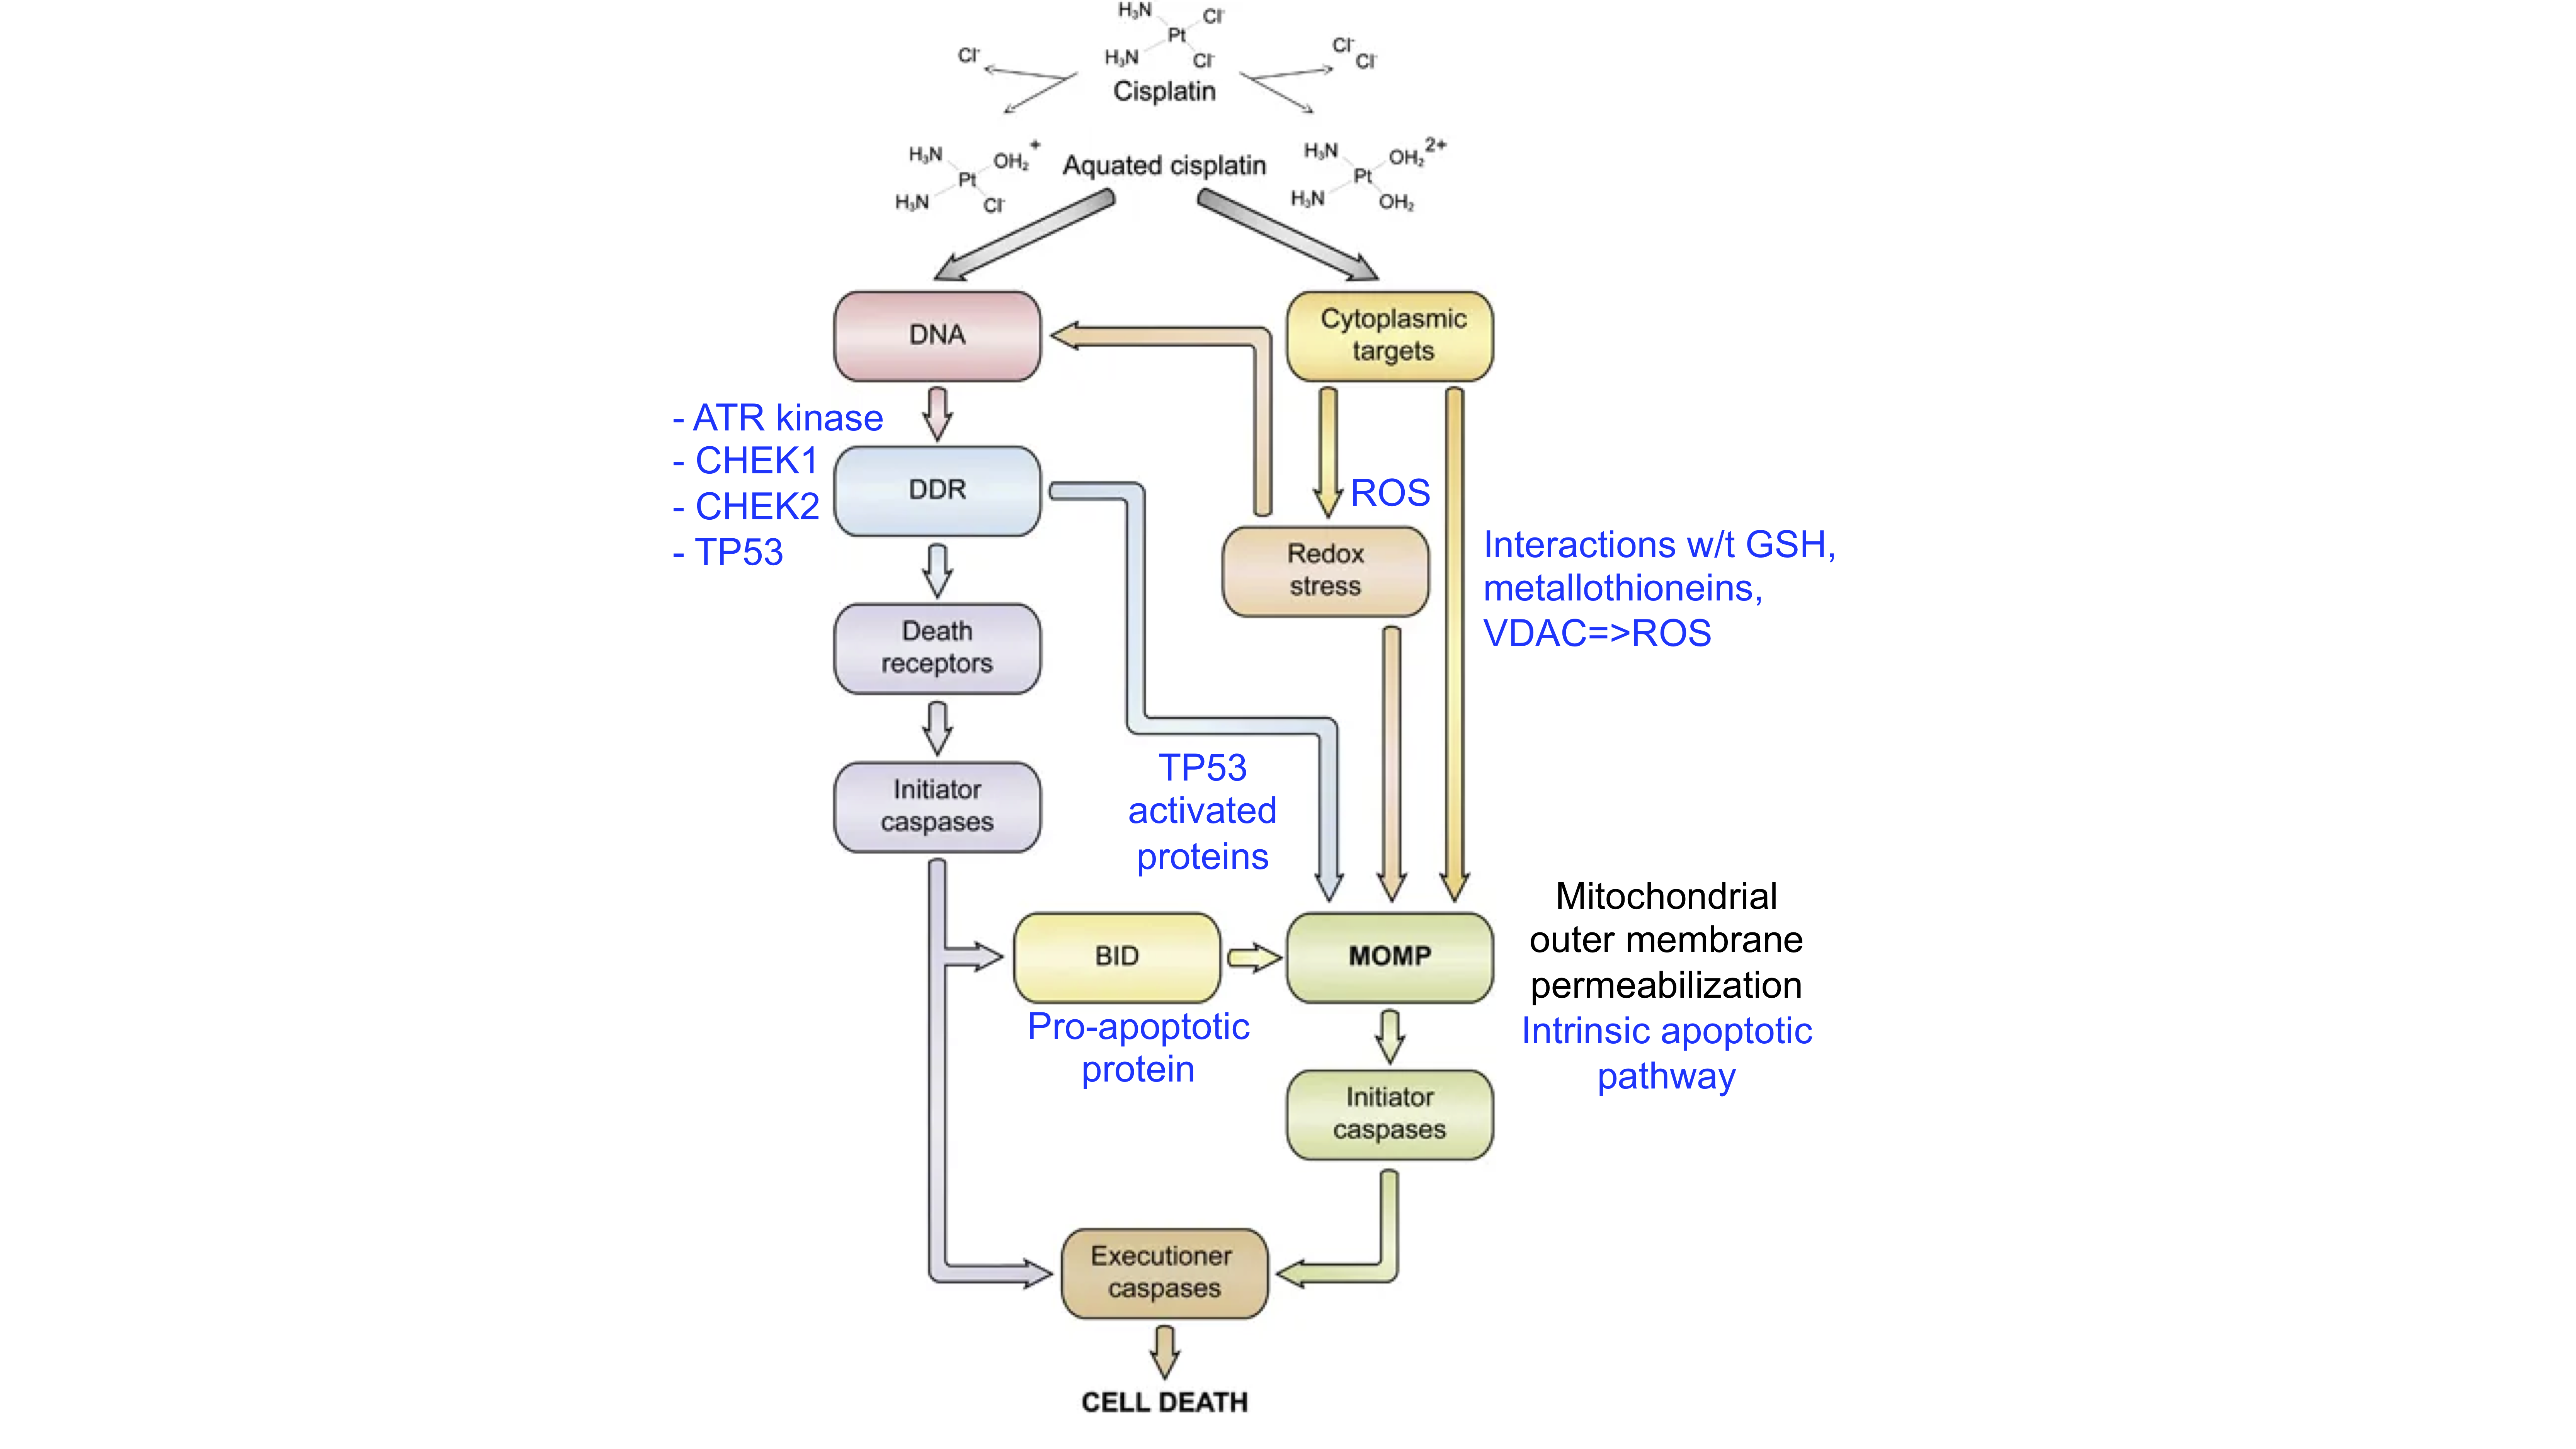
\includegraphics[width=\textwidth]{Figures/CisplatinMA.png}
	\caption[Mechanism of action of cisplatin]
	{\small
	    \textbf{Mechanism of action of cisplatin modified from \cite{galluzzi2012molecular}}.
	     Intra cellular cisplatin is rapidly aquated due to reduced cytoplasmic concentration of chloride ions. Aquated cisplatin binds to nuclear DNA, thereby promoting DNA damage rresponse.IN the cytoplasm, interact with several nucleophiles, including mtDNA as well as multiple mitochondrial and extracellular proteins causing formation of oxidative and reticular stress;provoking a signal transduction cascade that involves pro-apoptotic,BID, BCL-2 family members, as well as VDAC1 and activation of TP53 leading to MOMP and cell death.
	    TP53 activation could directly lead to Cell senescence not shown in the figure. MOMP, mitochondrial outer memberance permeabilization;BID, Bax-like BH3 protein; VDAC, Voltage-dependent anion channel; mtDNA, mitochondrial DNA.
	}
	\label{fig:CisplatinMA}
\end{figure}


The platinum atoms of cisplatin cross-links DNA by making covalent bonds with purine bases in particular with nucleophilic N7 sites. homotypic intra stand and low percentage of inter strand cross-links result in the generation of DNA-adducts that interfere with DNA replication and RNA transcription. If DNA is not repaired, DNA-damage induced cell-cycle arrest either becomes permanent (an oncosupressive response called senescence) or mitochondrial apoptosis is triggered \cite{fichtinger1985adducts, rabik2007molecular,lopez2013hallmarks}. 

%This effectiveness seems to be due to the unique properties of cisplatin, which enters cells via multiple pathways and forms multiple different DNA-platinum adducts while initiating a cellular self-defense system by activating or silencing a variety of different genes, resulting in genetic and/or epigenetic alterations.
The main signaling cascade that links cisplatin induced DNA lesions to apoptosis involves sequential activation of ATM and RAD3 related protein (ATR, a sensor of DNA damage) and checkpoint kinase 1 (CHEK1, is the downstream effector of ATR) that  eventually phosphorylates the tumor suppressor protein TP53 at serine 20  \textbf{\autoref{fig:CisplatinMA}} \cite{shieh2000human, cimprich2008atr}. Activated TP53 promotes mitochondrial outer membrane permeabilization (MOMP).  MOMP alone or with stimulatory signals via pro-apoptotic BCL-2 family (BID, BAK1, BAX) \cite {tajeddine2008hierarchical} sets off the caspase cascade dependent and independent mechanisms that leads to cell death. Checkpoint kinase 2 (CHECK2, is the downstream target of ATM), along with induces cell cycle arrest  (not cell death) through ATM signaling, also responds to cisplatin in an ATM-independent fashion \cite{pabla2008atr}. 

In the cytoplasm, the interaction of cisplatin with glutathione (GSH), metallothionines or mitochondrial proteins for example, voltage-dependent anion channel (VDAC), derives the generation of reactive oxygen species (ROS). ROS and nitric oxide (NO) exacerbate cisplatin toxicity along with increasing the opening of permeability transition pore complex (PTPC) on mitochondria \cite{godoy2012endogenously}. There are also evidence in literature that CHEK1 activates MAPK pathway signaling, mediated by extracellular signal-regulated kinases, c-JUN N-terminal kinases and stress-activated protein \cite{persons2000effect, yeh2002increase}.

\subsubsection{Mechanism of cisplatin resistance}
Cisplatin resistance can arise from transformation in the processes that precede the binding of cisplatin to its actual targets, including cytoplasmic structures and DNA. These factors are categorized as \textbf{pre-target resistance.} (See Summary \textbf{table 1.1)}) Briefly, copper transporter 1 (CTR1) mediate major fraction of cisplatin intake \cite{more2010role,ishida2010enhancing, holzer2006contribution}, whereas ATPase, copper transporting, beta polypeptide (ATP7B), is involved in cisplatin export \cite{katano2002acquisition,komatsu2000copper, aida2005expression}. Some plasma membrane transporters have been proposed to contribute to the extrusion of cisplatin, including ATP-binding cassette, subfamily C member 2, best known as multidrug  resistance-associated protein 2 (MRP2) \cite {cui1999drug,korita2010multidrug,liedert2003overexpression} and ATP-ase, class VI, type IIB (ATP11B) \cite{moreno2013atp11b}. Moreover, cisplatin resistant cells also exhibit high levels of metallothioneins \cite{kelley1988overexpression,kasahara1991metallothionein} and GSH, an enzyme that catalyzes GSH synthesis (i.e., gamma glutamylcysteine synthetase) and conjugates with cisplatin \cite{lewis1988glutathione,chen2010role}. 


\begin{table}[htbp]
   \centering
   \caption{Pre-target cisplatin resistance factors}
\begin{tabular}{p{1.5cm}p{5cm}p{5cm}p{1cm}}
\hline
\textbf{Genes/ Factors} & \multicolumn{1}{l}{ \textbf{Mode of Action}} & \multicolumn{1}{p{5cm}}{ \textbf{Importance}} & \multicolumn{1}{p{5cm}}{ \textbf{References}} \\ \hline

CTR1   & Reduced uptake, Plasma membrane copper transporter & Downregulated in resistant cells. CTR1 depletion increases cisplatin resistance. Copper chelators enhance the uptake and efficacy of cisplatin & \multicolumn{1}{p{5cm}}{ \cite{more2010role, ishida2010enhancing,holzer2006contribution,katano2002acquisition}} \\

ATP7A/ ATP7B & Increased efflux, Copper-extruding P-type ATPases involved in the regulation of ion homeostasis & Upregulated in cisplatin-resistant cells. ATP7B expression levels may predict the efficacy of cisplatin chemotherapy.  & \multicolumn{1}{p{5cm}}{\cite{katano2002acquisition,komatsu2000copper,nakayama2002copper,safaei2004role,aida2005expression}} \\ 

MRP2   & Increased efflux, Member of the ABC family of plasma membrane transporters. Mediates the ATP-dependent cellular efflux of cisplatin. & Overexpressed in cisplatin-resistant cells. Modulation by antisense cDNA enhances cisplatin sensitivity. Expression levels affect the efficacy of cisplatin regimens. & \multicolumn{1}{p{5cm}}{\cite{cui1999drug,korita2010multidrug,liedert2003overexpression, yamasaki2011role}} \\

GSH/ GCS/ GST & Increased inactivation, GSH scavenges electrophiles and ROS. GCS catalyzes GSH synthesis. GST conjugates GSH to cisplatin and facilitates its extrusion. & Resistant cells often exhibit high levels of GSH, GCS and GST.  & \multicolumn{1}{p{5cm}}{\cite{lewis1988glutathione,chen2010role}} \\

Metallo-thionein & Increased inactivation, Intracellular thiol-containing proteins involved in the detoxification of metal ions. & May bind and inactivate cisplatin.  & \multicolumn{1}{p{5cm}}{\cite{kelley1988overexpression,kasahara1991metallothionein}} \\   \hline
\end{tabular}%
\begin{tablenotes}
\small
      \item  {CTR1,copper transporter receptor 1; MRP, multi-drug resitance proteins; ROS, reactive oxygen species; GSH, glutathione; GCS,gamma-glutamylcysteine synthetase; GST, glutathione S-transferases}.
    \end{tablenotes}
 
   \label{tab:addlabel}%
 \end{table}%


The mechanism of \textbf{on-target cisplatin resistance} is believed to arise in particular with the removal of cisplatin DNA-adducts and subsequent apoptosis can be defective in cisplatin-resistant cancer cells due to a variety of mechanisms including \ac{NER} proficiency \cite{wood2000dna, shuck2008eukaryotic}. They are summarized in \textbf{table 1.2}. In addition, another proposed mechanism for cisplatin resistance involves high expression of the high-mobility group box protein 1 (HMGB1), that appears to bind selectively to cisplatin DNA crosslinks and interferes with \ac{NER} while HMGB3 is associated with the promoter regions of ATR and CHK1 \cite{awuah2017repair, mukherjee2019targeting}. 




\begin{table}[htbp]
   \centering
   \caption{On-target cisplatin resistance factors}
    \begin{tabular}{p{1.5cm}p{5cm}p{5cm}p{1cm}}
     \hline
      \textbf{Genes/ Factors} & \multicolumn{1}{l}{ \textbf{Mode of Action}} & \multicolumn{1}{p{5cm}}{ \textbf{Importance}} & \multicolumn{1}{p{5cm}}{ \textbf{References}} \\ \hline
ERCC1  & Increased NER proficiency, Single-strand endonuclease, in association with ERCC4/XPF incises DNA on the 5′ side of cisplatin adducts. & ERCC1 expression negatively correlates with  cisplatin clinical responses in multiple human cancers & \multicolumn{1}{p{5cm}}{Dabholkar et al., 1992;Metzger et al., 1998;Shirota et al., 2001;Olaussen et al., 2006;Handra-Luca et al., 2007;Bellmunt et al., 2007;Kim et al.,} \\
MLH1 & MMR deficiency, Component of a multiprotein complex that excides and repairs DNA mismatches.Implicated in DNA damage signaling and apoptosis. & MLH1 deficiency is sometimes associated with  cisplatin resistance (and increased TLS).  & \multicolumn{1}{p{5cm}}{Nakayama et al., 2002;?Nakayama et al., 2004;Safaei et al., 2004;Aida et al., 2005} \\ MSH2  & Forms heterodimers that detect DNA lesions including base–base mismatches. & Low MSH2 levels predict  cisplatin benefits in patients with resected lung cancer. & \multicolumn{1}{p{5cm}}{Koike et al., 1997;Cui et al., 1999;?Liedert et al., 2003;Korita et al., 2010;?Yamasaki et al., 2011} \\POLH & Increased TLS, DNA polymerase that substitutes stalled replicative polymerases and includes nucleotides opposite to the DNA lesion. & POLH upregulation correlates with short patient survival. & \multicolumn{1}{p{5cm}}{Lewis et al., 1988;?Chen and Kuo, 2010} \\
REV3/ REV7 & Catalytic (REV3) and structural (REV7) subunits of the TLS DNA polymerase . & REV3 defects correlate with increased cisplatin sensitivity in cancer cell lines. REV overexpression is associated with  cisplatin resistance  & \multicolumn{1}{p{5cm}}{Wittschieben et al., 2006;Shachar et al., 2009;Roos et al., 2009} \\  
BRCA1/ BRCA2 & Increased HR proficiency, HR DNA repair. Regulation of transcription and cell cycle progression. & BRCA1/2-deficient tumors respond better to  cisplatin. Secondary mutations that restore BRCA function favor acquired chemoresistance.& \multicolumn{1}{p{5cm}}{Narod and Foulkes, 2004;Edwards et al., 2008;Sakai et al., 2008}  \\  
VDAC & Cisplatin binding proteins, protein of the OM that mediates vital functions but also participates into the PTPC.& Depletion/or inhibition of VDAC increases  cisplatin resistance. Might also be involved in post-target resistance.& \multicolumn{1}{p{5cm}} {Yang et al., 2006;Kroemer et al., 2007;Tajeddine et al., 2008}\\  
    \hline
     \end{tabular}%
  \begin{tablenotes}
      \small
      \item  {ERCC1, excision repair cross-complementing rodent repair deficiency, complement group1, HR, homologous recombination; TLS, translesion synthesis; OM, mitochondrial outer membrane; XPF, xeroderma pigmentosum complementation group; VDAC, voltage dependent anion channel; PTPC, permeability transition pore complex.}
    \end{tablenotes}
 
   \label{tab:addlabel}%
 \end{table}%



\begin{figure}
\centering
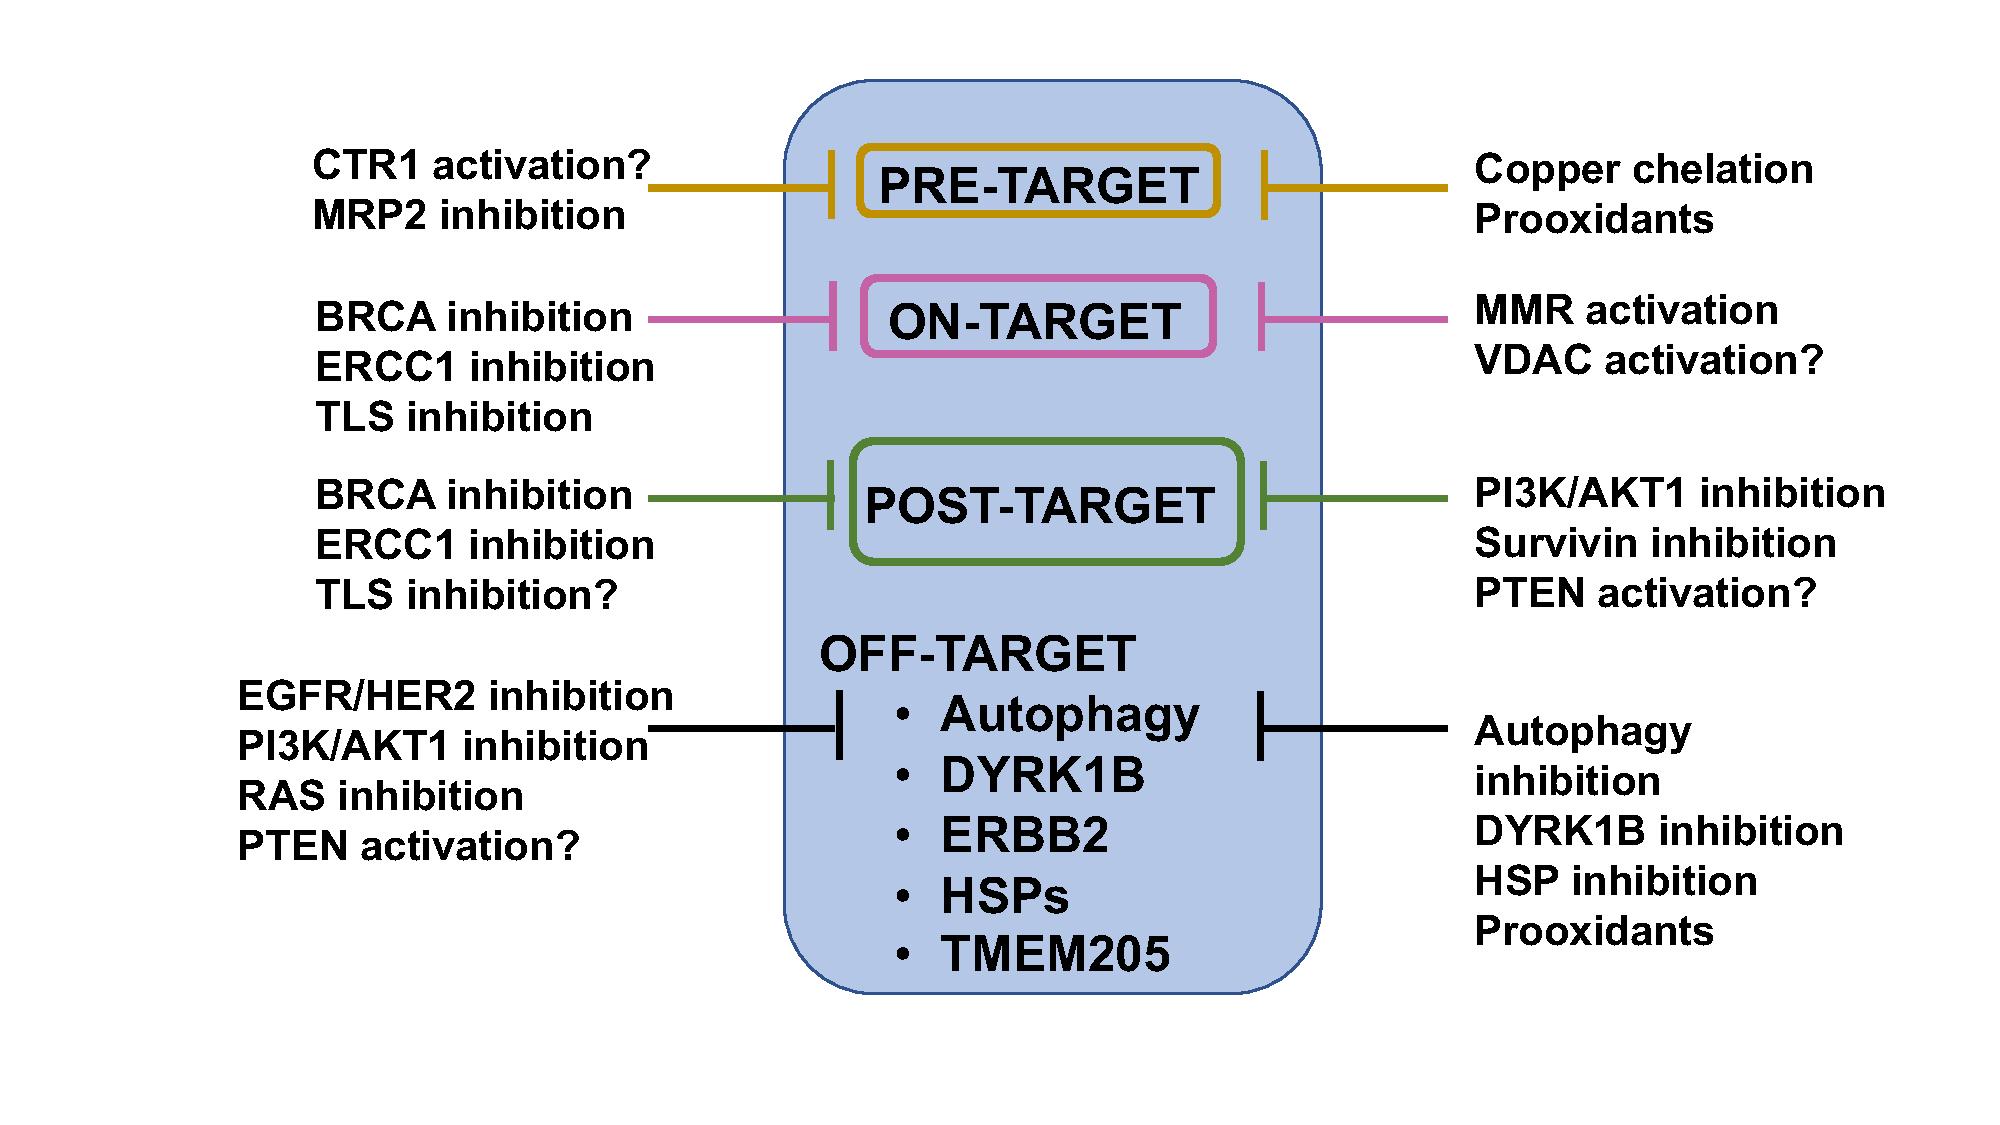
\includegraphics[width=\textwidth]{Figures/circumventingcisplatinresistance.pdf}
	\caption[Mechanism of action of cisplatin]
	{\small
	    \textbf{Strategies for reverting cisplatin resistance. Modified from  \cite{galluzzi2012molecular}}.
	     Cisplatin resistance most often has a multifactorial nature, implying that targeting one mechanism of resistance at a time has very low chances to result in significant chemosensitization. Thus, combination strategies for blocking cisplatin resistance at multiple levels should be designed. With regard to this, detailed information on the patient genetic and epigenetic background might be critical for determining which specific mechanisms should be targeted to fully circumvent chemoresistance. EGFR, epidermal growth factor receptor; HSP, heat-shock protein; PTEN, phosphatase and tensin homolog; TLS, translesion synthesis.
	}
	\label{fig:circumventingcisplatinresistance}
\end{figure}



\textbf{Post-target resistance} to cisplatin can result from alterations in signal transduction pathways that mediate apoptosis in response to DNA damage. Non-repairable cisplatin-induced DNA damage leads to the activation of a multi-branched signaling cascade with proapoptotic outcomes. Several groups have provided evidence that predominant mechanisms involves the inactivation of \textit{Tp53}, which exists in around half of all human cancers \cite{kirsch1998tumor}. Reportedly patients harboring wild-type \textit{Tp53} have a higher probability to take advantage from cisplatin as compared to the patients with \textit{Tp53} mutations \cite{vousden2007p53,gadducci2002molecular}. 
Furthermore, inhibition of PDGFRβ mediated phosphorylation of AKT by Ly294002 reversed cisplatin resistance \cite{juliachs2014pdgfrbeta}. Somatic mutations within PI3KCA, AKT and FGFR3 were also reported in cisplatin resistance \cite{feldman2014presence}. Pre-clinical studies indicate that targeting PDGFR/PI3K/AKT pathway  pathway may reverse cisplatin resistance \cite{juliachs2013effectivity}.
Upregulation of IGF1R expression and signaling was also found to contribute to acquired cisplatin resistance \cite{selfe2018igf1r}. 

Variations in any of the factors that regulate and carry out apoptosis have the potential to influence cisplatin sensitivity. It could be triggered by DNA damage or oxidative stress via the mitochondrial pathway. Numerous proteins including death receptors, cytoplasmic adaptors. pro- and antiapoptotic members of the BCL-2 family, caspases, calpains and many others \cite{jain2011molecular, janson2010resistance, michaud2009bcl}. Ryan \textit{et al} reported that BIRC5 (Survivin) overexpression is associated with chemoresistance and poor prognosis in multiple types of cancer \cite{ryan2009survivin}. 

Cisplatin-resistant phenotype can also be sustained through \textbf{off-target resistance} including the alterations in signaling pathways that are not directly engaged by cisplatin. Relavant factors include are autophagy \cite{tan2019trp14}, DYRK1B \cite{hu2010depleting}, ERBB2 \cite{fijolek2006p53}, HSP \cite{ren2008down} and TMEM205 \cite{shen2010elevated}.


\subsubsection{Strategies for circumventing cisplatin resistance}
As summarised above, there are at least four distinct but broad categories of mechanisms by which cancer cells become resistant to cisplatin. The major hurdle to overcome this clinically relevant issue is that often more than one resistance mechanism is activated thus exhibiting a multifactorial nature of cisplatin resistance.  \textbf{\autoref{fig:circumventingcisplatinresistance}} is summarizing some potential strategies of overcoming cisplatin resistance. 


\subsection{CX-5461: G4 stabilizer} 
CX-5461 is a small molecule G-quadruplex stabilizing compound. It was developed as a selective RNA polymerase I inhibitor \cite{drygin2011targeting}. Recent evidence suggests that it causes DNA damage and induce selective lethality in BRCA1/2 deficient tumours \cite{xu2017cx}, resulting in a first in human Canadian clinical trial (CCTG-IND231). 
 
 \subsubsection{G-quadruplex structures}
G-quadruplex (G4) structures arise transiently at guanine-rich sequences in the folded DNA and RNA, when two or more G-tetrads stack on top of each other and coordinate monovalent cations, such as K+ and Na+ \cite{sen1990sodium} \textbf{\autoref{fig:G4structures} a}. Each tetrad is composed of four G residues that are linked by the sugar–phosphate backbone and connected through Hoogsteen-type hydrogen bonds \cite{kwok2017g}. G-quadruplex structures can fold intramolecularly from a single G-rich strand, or intermolecularly through dimerization or tetramerization of separate filaments. They both can present prarallel or anti parallel topologies \textbf{\autoref{fig:G4structures} b}. The length of loop can vary (1-7 nucleotides), with smaller loops being more stable\cite{huppert2010structure}.
G4 sequences mainly clustered in central genomic regions, namely single-stranded 3’ overhangs in telomeres, gene promoters, especially oncogenes and DNA replication origins. In cancer cells these structures are important in DNA replication, telomere maintenance, and regulation of transcription and transplation \textbf{\autoref{fig:G4structures} c, d, e} \cite{rhodes2015g, maizels2013g4}. Literature based on large scale DNA sequencing on human genome have revealed over 700,000 putative G4 sites and 10,000 of them have been identified from ChIP-seq using an antibody that recognises G4 structures \cite{siddiqui2002direct, granotier2005preferential, chambers2015high, hansel2016g}.

 \begin{figure}
\centering
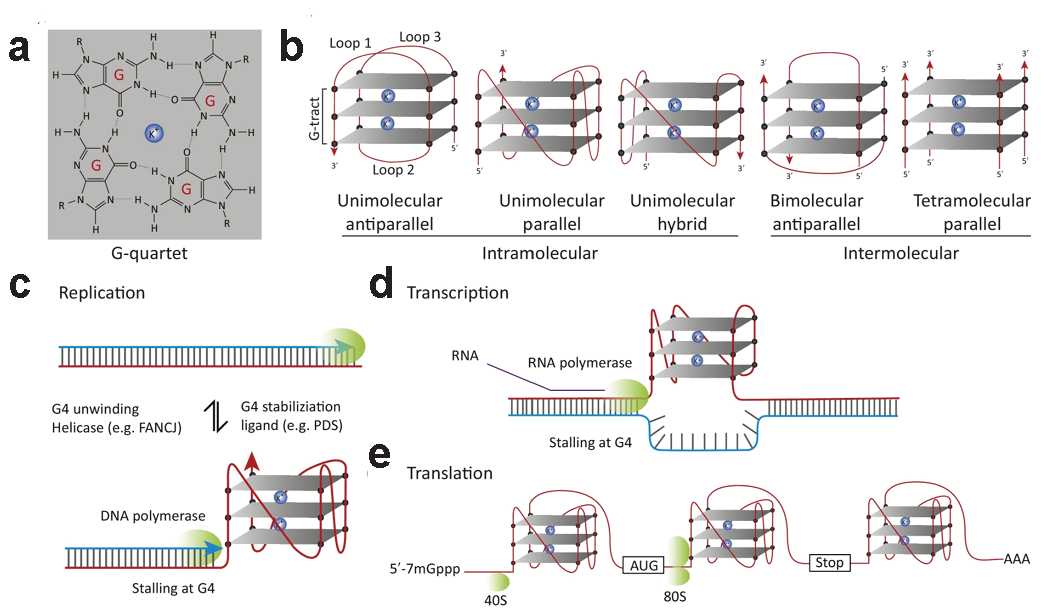
\includegraphics[width=\textwidth]{Figures/G4structures.pdf}
	\caption[The G4 structures and their biology]
	{\small
	    \textbf{The G4 structures and Biology. Modified from \cite{kwok2017g}}.
	   \textbf{(a)} Chemical structure of a G-quartet. Potassium ion (K+) sits within the G-quartet for stabilization. G-quartets stack on each other to form G-quadruplex \textbf{(b)} Representative topologies of G-quadruplex structures. \textbf{(c-e)} Representative G-quadruplex-associated biology: regulation of \textbf{(c)} DNA replication, \textbf{(d)} transcription, and \textbf{(e)} translation
	}
	\label{fig:G4structures}
\end{figure}
 
 
 \subsubsection{CX-5461 leads to synthetic lethality with  DNA repair pathways deficiency}
 The dominant feature of the p53/basal expression group of TNBC is genomic instability \cite{yu2013identification}. It is essential to identify specific subgroups that could be targeted through synthetic lethal approaches, analogous to PARP inhibitors that exploit loss of homologous recombination repair (HR) \cite{fong2009inhibition}.
 CX-5461, in addition to polymerase 1 inhibition and G4 stabilization, has been recently shown to have activity in \ac{HR} and \ac{NHEJ} deficient cancer cells \cite{zimmer2016targeting,xu2017cx}. 
 BRCA1/2 deficiency leads to compromised HR repair, generating an increased error-prone DNA repair and ultimately, genomic instability. The BRCA2/RAD51 complex is also involved in many other aspects of genome instability, such as stalled DNA replication fork stabilization \cite{schlacher2011double}, R-loop resolution \cite{bhatia2014brca2} and repairing G-quadruplex (G4) associated DNA damage .
 Studies have shown that stabilization of G-quadruplex forming regions of the genome results in synthetic lethality in DNA repair deficient cancers including HRD, non-homologous end joining (NHEJ) \cite{xu2017cx, mcluckie2013g, zimmer2016targeting}. 
The study by Xu \textit{et al}. also benefited from some of the CX-5461 drug efficacy \textit{in vitro} experiments performed for chapter 3 of this thesis \textbf{(\autoref{fig:invitro} c)}, exploring \ac{NHEJ} pathway involvement.  
We reported that both CX-5461 and the related compound CX-3543 induce DNA damage and are dependent on BRCA1/2-mediated HR and DNA-PK-mediated NHEJ pathway for damage repair \cite{xu2017cx}.

%%%%%%%%%%%%%%%%%%%%%%%%%%%%%%%%%%%%%%%%%%%%%%%%%%%%%%%%%%%%%%%%%%%%%%

\section{Single cell sequencing can reveal molecular dynamics of cellular
population fitness in patients and model systems}
Cellular fitness underpins the tissue population dynamics of cancer progression and treatment response. Yet, quantifying fitness in heterogeneous cell populations and identifying causal mechanisms shaping fitness landscapes remain open problems, impeding progress in developing effective and durable therapeutic strategies. In particular, quantitative fitness modelling of cancer cells has numerous and diverse implications; attributing clonal dynamics to drift or selection, identifying the determinants of clonal expansion, enabling causal inference, and forecasting growth trajectories. 

Large scale single cell genome measurements to scalably define clonal populations in  cancer  over  thousands  of  cells  have  only  recently  emerged,  enabling  identification  of rare populations, precise tracking of clones and robust clone-specific measurements suitable for population genetics modeling  \cite{laks2019clonal,zahn2017scalable}. Several amplification-based methods have been described \cite{navin2011tumour,zong2012genome, hou2012single,ni2013reproducible} but measuring single-cell genomes at \ac{DLP+} in tissues and cell populations has greatly advanced clonal decomposition of malignant tissues. Moreover, helped studying properties of negative selection, resolving rare cell population genotypes and identifying DNA replication states of individual cells, all of which are hard to measure when cellular information is destroyed in bulk sequencing. 
From DLP+ variation in mitotic mis-segregation rates across tissue types and genotypes can be defined. Analysis of matched genomic and image measurements can reveal correlations between cellular morphology and genome ploidy states. Aggregation of cells sharing copy number profiles allowed for calculation of single-nucleotide resolution, clonal genotypes and inference of clonal phylogenies.

\subsection{Identification of sub-population in growing cancers}
To quantify fitness based on sub-population in growing cancers require 

(i) method for identifying sub-populations with their genotypes
(ii) serial sampling of the populations
(iii) a method for estimating the likelihood the trajectory is non neutral

Limitations of this approach to structural and copy number genotypes arise from inability to resolve populations accurately. Single cell sequencing technology opens up the opportunity to accurately identify CNA, structural sub-populations
We know from population genetics that it is possible to measure quantitatively the tendency of populations with shared genotypes to experience differential growth and survival, i.e. the \textbf{fitness of genotypes}, from population samples drawn \textbf{over time}.
These two concepts can be linked to measure the fitness associated with copy number assigned clones identified by a novel scWGS method (DLP+), in serially sampled tumours.
\subsection{Statistical models to quantify fitness of clones}
Two key statistical innovations were required, a Bayesian phylogenetic inference method, \textbf{Sitka} that scales to thousands of cells for copy number states in scWGS and adaptation of a birth death process statistical model, and  \textbf{Wright-Fisher diffusion}, to scWGS genotypes, named as \texttt{fitClone}.

\subsubsection{Introduction to Sitka application on single cell data}


\subsubsection{\texttt{fitClone}-quantitative measure of fitness model}




\section{Studying cancer dynamics by single cell RNA sequencing}
For any given difference between the types of drug resistance, for example, the expression of a particular gene, it is assumed that differences arise deterministically or probabilistically in the configuration of transcription factors regulating the genes in the tumors. Cancer cells in distinct cell- states often exhibit important differences in functional properties depending on the which genes are turned on and off resulting in sensitive or resistant phenotype.

The most challenging analysis is to differentiate whether the change in gene expression leading to change in cellular state is stochastic \cite{raj2008nature} and random or its deterministic to produce the same output under similar environment.
Cancer cells in distinct cell- states often exhibit important differences in functional properties depending on which genes are turned on and off resulting in sensitive  or resistant phenotype.
Previously it is shown that unique cells within a population can exhibit fluctuations in expression of a group of genes, that could predict distinct phenotypes \cite{shaffer2020memory}.
Un-like genomic clones that could get selected in resistant phenotype \cite{salehi2020single}, we still are not clear whether the cell-states are acquainted for this kind of behaviour or the selected states are pre-existing in the cancer population and under continues pressure shows obvious dynamics or there is a transition from one state to another that ultimately gets selected over time. Because of difficulty to analyse longitudinal patient's samples for single cell gene expression and lack of multiple longitudinal pre-clinical breast cancer models, these questions remains unexplored.

\subsection{Linking gene expression states to cancer clones}
(From clonealign paper) Recent advances in genomic measurement technologies have allowed for unprecedented scalable interrogation of the genomes and transcriptomes of single cells \cite{zahn2017scalable, zheng2017massively}. Such technologies are of particular interest in cancer, enabling measurement of cell-autonomous properties which constitute tumors as a whole. Molecular phenotyping at the single-cell level enables reconstruction of tumor life histories through phylogenetic analysis \cite{jahn2016tree, smith2017scape}, and quantification of intra-tumoral heterogeneity and its clinical implications \cite{tellez2016tumour,mitra2014single}.

Theoretically, combined assays sequencing both RNA and DNA from the same single cell will provide a measurement of genomic alterations impacting transcriptional programs. This would yield a powerful single-cell level genotype-phenotype read out. We have used recently published tool, clonealign, that can perform statistical integration of independent single-cell RNA-seq and DNA-seq from patient derived xenograft tumors \cite{campbell2019clonealign}.  


%%%%%%%%%%%%%%%%%%%%%%%%%%%%%%%%%%%%%%%%%%%%%%%%%%%%%%%%%%%%%%%%%%%%%%
\section{Thesis goals and Scientific questions}
Drug resistance and etiology are among the key unresolved areas of investigation that require advanced understanding of fitness in cancer. For example, drug resistance mechanisms are commonly attributed to phenotypic plasticity encoded via epigenetic changes \cite{shaffer2017rare,sun2014reversible} or evolutionary selection of pre-existing genomic clones \cite{vasan2019view}. However, the relative contribution of these processes when  studied  in  tandem  is  poorly  understood  and  requires  integrated  genome-transcriptome investigation.   Moreover,  how  changes  in  genomic  architecture  brought  about  by  copy  number alterations drive etiologic processes remains understudied. Perturbations to induce fitness changes include genetic editing with cancer gene mutations, and pharmacologic drug selection to profile kinetics of therapeutic response.

The goal of this thesis is to develop timeseries models with and without  drug perturbation and undertake integrated  genome-transcriptome investigation to quantify fitness in cancer population at single cell level. 
Fitness based on sub-population analysis requires:
- method for identifying sub-populations with their genotypes
- serial sampling of the populations
- a method for estimating the likelihood the trajectory is non neutral
Limitations of this approach to structural and copy number genotypes arise from inability to resolve populations accurately.
Recent development of single cell sequencing methods opens up the opportunity to accurately identify \ac{CNA}, structural sub-populations
In this thesis, we have used all different types of breast tumors for testing transplant capability and initial screening in chapter 3.  However, for chapter 4 and chapter 5 exclusively all \ac{TNBC} were selected to create timeseries forced amplified evolution models under chemotherapy selection.
to determine the cellular mechanisms in resistance  at single cell resolution.

 We have used \ac{scWGS} and \ac{sc-RNAseq} to define the population dynamics in re-transplantable TNBC PDX.
 Since TNBC PDX are especially dynamic and exhibit genomic instability, a longitudinal tracking of tumor passages in PDX provides insights into the stability of genome instability patterns, as well as clonal transcriptional states over genomic clones.
 
 In \textbf{Chapter 3}, we established a transplant model and the methods for single cell dissociation. PDX generations, protocol development, optimizations and \textit{in vivo} screening. 
 
 In \textbf{Chapter 4}, Identifying patterns of clonal resistance with single cell whole genome sequecning. 
 
 In \textbf{Chapter 5}, We identified resistance phenotypes by longitudinal scRNA sequencing and characterization of differentially  expressed genes and pathways 

